\pdfoutput=1
\RequirePackage{ifpdf}
\ifpdf % We~are running pdfTeX in pdf mode
\documentclass[pdftex]{sigma}
\else
\documentclass{sigma}
\fi

\numberwithin{equation}{section}

\newtheorem{Theorem}{Theorem}[section]
\newtheorem*{Theorem*}{Theorem}
\newtheorem{Corollary}[Theorem]{Corollary}
\newtheorem{Lemma}[Theorem]{Lemma}
\newtheorem{Proposition}[Theorem]{Proposition}

\theoremstyle{definition}
\newtheorem{Definition}[Theorem]{Definition}
\newtheorem{Note}[Theorem]{Note}
\newtheorem{Example}[Theorem]{Example}
\newtheorem{Remark}[Theorem]{Remark}
\newtheorem*{Remark*}{Remark}

\def\w{\omega}
\def\tentt{\tt}
\newcommand{\qbin}[2]{\left[\begin{matrix} #1 \\ #2 \end{matrix} \right]}
\newcommand{\bin}[2]{\left(\begin{matrix} #1 \\ #2 \end{matrix} \right)}

\begin{document}
\allowdisplaybreaks

\newcommand{\arXivNumber}{2507.14734}

\renewcommand{\thefootnote}{}

\renewcommand{\PaperNumber}{104}

\FirstPageHeading

\ShortArticleName{Basis Partitions and Their Signature}

\ArticleName{Basis Partitions and Their Signature\footnote{This paper is a~contribution to the Special Issue on Basic Hypergeometric Series Associated with Root Systems and Applications in honor of Stephen C.~Milne's 75th birthday. The~full collection is available at \href{https://www.emis.de/journals/SIGMA/Milne.html}{https://www.emis.de/journals/SIGMA/Milne.html}}}

\Author{Krishnaswami ALLADI}

\AuthorNameForHeading{K.~Alladi}

\Address{Department of Mathematics, University of Florida, Gainesville, FL 32611-8105, USA}
\Email{\mail{alladik@ufl.edu}}
\URLaddress{\url{https://people.clas.ufl.edu/alladik/}, \url{http://krishnaswami-alladi.com/}}

\ArticleDates{Received July 23, 2025, in final form November 28, 2025; Published online December 11, 2025}

\Abstract{Basis partitions are minimal partitions corresponding to successive rank vectors. We show combinatorially how basis partitions can be generated from primary partitions which are equivalent to the Rogers--Ramanujan partitions. This leads to the definition of a~signature of a basis partition that we use to explain certain parity results. We then study a special class of basis partitions which we term as complete. Finally, we discuss basis partitions and minimal basis partitions among partitions with non-repeating odd parts by representing them using 2-modular graphs.}

\Keywords{basis partitions; Rogers--Ramanujan partitions; Durfee squares; sliding operation; signature; partial theta series}

\Classification{05A17; 05A19; 05A15}

\renewcommand{\thefootnote}{\arabic{footnote}}
\setcounter{footnote}{0}

\rightline{\it Dedicated to Steve Milne on the occasion of his 75th birthday}

\section{Introduction}

For a partition $\pi\colon b_1\ge b_2\ge \dots \ge b_\nu$, its Ferrers graph
is an array of left-justified rows with $b_i$ nodes in the $i$-th row,
$i=1,2,\dots,\nu$.
The conjugate $\pi^*$ of $\pi$ is
obtained
by counting the nodes in the columns of the Ferrers graph of $\pi$.
Let
$\pi^*$ be $c_1\ge c_2 \ge \dots \ge c_{b_1}$.

In every Ferrers graph, there is a largest square of nodes called the
{\it Durfee square} which is the same for the conjugate as well. Given
a partition $\pi$ as above, let it have a $k\times k$ Durfee square.
The successive rank vector of $\pi$ is defined as $\mathbf{r}= (r_1, r_2, \dots ,
r_k)$, where
\begin{equation*}
r_i=b_i-c_i \qquad \text{for} \ i=1,2,\dots,k. %\label{eq:1.1}
\end{equation*}

Note that $r_1=b_1-c_1$ is the {\it rank} that Dyson~\cite{Dy44} used
to combinatorially explain two of Ramanujan's congruences. This led
to the terminology {\it successive ranks} for the differences $b_i-c_i$
which are equal to hook differences. Their study has led to the discovery of
important partition identities, the results in Andrews et al.~\cite{An-Ba-etal0087} being a good
example.

Given $\mathbf{r}$, there are, in general, several partitions $\pi$
which will have $\mathbf{r}$ as the successive rank vector. Among all
partitions $\pi$ having a prescribed successive rank vector, consider
the partition for which the sum of the parts $\sigma(\pi)=b_1+b_2+\dots +
b_{\nu}$ (the integer being partitioned) is minimal. Gupta~\cite{Gu0076} called
such minimal partitions as {\it basis partitions} and proved their
existence. He also noticed that if $\pi$ is the basis partition associated
with a rank vector $\mathbf{r}= (r_1, r_2, \dots , r_k)$ and if~${n>\sigma(\pi)}$, then the number
of partitions of $n$ which have the same rank vector $\mathbf{r}$ is equal to
the number of partitions of $(n-\sigma(\pi))/2$ into $\le k$ parts.

We provide here a combinatorial procedure to generate basis
partitions from primary partitions which are equivalent to the
Rogers--Ramanujan partitions (see Section~\ref{section3}), and use that for a new study
of basis
partitions among partitions with non-repeating odd parts (Section~\ref{section9}).
Hirschhorn~\cite{Hi0099} had noticed
that the number of basis partitions of an integer $n$ can be expressed
as a weighted count over the Rogers--Ramanujan partitions of $n$, where
the weights are powers of~2. He deduced this by suitable interpretation
of the generating function of basis partitions obtained by Nolan, Savage,
and Wilf~\cite{No-Sa-Wi0098}.

Our approach provides a very natural combinatorial proof of
Hirschhorn's weighted identity
as well as a refinement of the generating function of basis
partitions that leads to a statistic which we call the {\it signature}.
A study of the parity of the signature yields a partial theta series involving
the squares (Section~\ref{section5}). This parity result has nice
counterparts for partitions with non-repeating odd parts (Section~\ref{section9}).

\section{The generating function of basis partitions}\label{section2}

The Ferrers graph of any partition $\pi$ may be split into three
parts as follows: (i)~the Durfee square $D(\pi)$, (ii)~the partition
$\pi_r$ which is the part to the right of the Durfee square, and
(iii)~the partition $\pi_b$ which is the portion below the Durfee
square. If in a partition there is a column of $\pi_r$ which is
equal in length to a row of $\pi_b$, then we may remove this
row and column to get a~smaller partition which will have the
same successive rank vector. Thus, a basis partition, by definition
of its minimality, will not have such a redundancy. Thus, we have
the following:

{\bf Characterization.} \textit{$\pi$ is a basis partition
if and only if no column of $\pi_r$ equals any row of~$\pi_b$.}
Conversely, given a basis partition with rank vector $\mathbf{r}$
of length~$k$, all partitions having the same rank vector can be
generated by inserting columns of length $\le k$ to the right of
the Durfee square, and inserting rows below the Durfee square
exactly equal in length and multiplicity to the inserted columns.
This observation can be used to compute the generating function
of basis partitions.

Let $b(n;k)$ denote the number of basis partitions whose rank vector
is of length $k$. Let $p(n;k)$ denote the number of partitions
having a $k\times k$ Durfee square. It is well known that
\begin{equation}
\sum_{n}p(n;k)q^n=\frac{q^{k^2}}{\bigl\{(1-q)\bigl(1-q^2\bigr)\cdots \bigl(1-q^k\bigr)\bigr\}^2}.\label{eq:2.1}
\end{equation}
Also, from the observation in the preceding paragraph, we have
\begin{equation}
\sum_{n}p(n;k)q^n=\frac{1}{\bigl(1-q^2\bigr)\bigl(1-q^4\bigr)\cdots \bigl(1-q^{2k}\bigr)}
\sum_{n}b(n;k)q^n.\label{eq:2.2}
\end{equation}
From~\eqref{eq:2.1} and~\eqref{eq:2.2}, it follows that
\begin{equation}
\sum_{n}b(n;k)q^n=\frac{q^{k^2}(1+q)\bigl(1+q^2\bigr)\cdots \bigl(1+q^k\bigr)}
{(1-q)\bigl(1-q^2\bigr)\cdots \bigl(1-q^k\bigr)}.\label{eq:2.3}
\end{equation}

The derivation of~\eqref{eq:2.3} given above is due to Hirschhorn~\cite{Hi0099}.
In~\cite{No-Sa-Wi0098}, the above characterization of basis partitions is observed,
but the derivation of~\eqref{eq:2.3} is by other means. Andrews~\cite{An2015} has studied basis partitions and a certain polynomial associated with~\eqref{eq:2.3}, but he interpreted~\eqref{eq:2.3} in terms of overpartitions.

Rogers--Ramanujan partitions $\pi\colon b_1+b_2+\dots +b_k$ are those whose
parts differ by at least 2. That is,
\begin{equation*}
b_i-b_{i+1}\ge 2, \qquad \text{for} \ i=1,2,\dots , k-1.%\label{eq: 2.4}
\end{equation*}
It is well known~\cite{An-book} that the generating function of the Rogers--Ramanujan
partitions into exactly~$k$ parts is
\begin{equation}
\frac{q^{k^2}}{(1-q)\bigl(1-q^2\bigr)\cdots \bigl(1-q^k\bigr)}.\label{eq:2.5}
\end{equation}
The way one realizes this is to note that the minimal partition into
$k$ parts differing by~\mbox{$\ge 2$} is~$1+3+5+\dots + (2k-1)=k^2$. This accounts
for the term \smash{$q^{k^2}$} in the numerator in formula~\eqref{eq:2.5}. One can construct all
partitions into $k$ parts that differ by $\ge 2$ from the minimal partition
by inserting columns of length $\le k$ into the Ferrers graph. This accounts
for the factors ${(1-q)\bigl(1-q^2\bigr)\cdots \bigl(1-q^k\bigr)}$ in the denominator in~\eqref{eq:2.5}.

Hirschhorn~\cite{Hi0099} notes that since
\begin{equation*}
\frac{\bigl(1+q^j\bigr)}{\bigl(1-q^j\bigr)}=1+2\bigl(q^j+q^{2j}+\dots +q^{nj}+\cdots \bigr),%\label{eq:2.6}
\end{equation*}
the insertion of the columns of a given length $j$ into the minimal
partition increases the size of the gap and the increase is to be counted
with weight~2. Thus, he deduces the following.

\begin{Theorem}[{Hirschhorn~\cite{Hi0099}}]\label{thm:1}
Let $\mathbf{R}$ denote the set of Rogers--Ramanujan partitions. For
each partition $\pi\in \mathbf{R}$,
\begin{equation}
\pi\colon\ b_1+b_2+\dots +b_k, \qquad b_i-b_{i+1}\ge 2 \quad \text{for} \
i=1,2,\dots , k-1, \ \text{and} \ b_k\ge 1, \label{eq:2.7}
\end{equation}
let its weight be $\omega(\pi)=2^t$, where t is the number of
strict inequalities in~\eqref{eq:2.7}. Then
\[
b(n,k)=\sum_{\pi\in \mathbf{R},\, \sigma(\pi)=n,\, \nu(\pi)=k}\omega(\pi).
\]
Here $\nu(\pi)$ denotes the number of parts of a partition~$\pi$.
\end{Theorem}

\section{Constructing basis partitions from primary partitions}\label{section3}

We define a {\it primary} partition $\pi$ to be one for which $\pi_b$ is
empty, that is, there are no nodes below the Durfee square. It is well known
\cite{An-book} that the expression in~\eqref{eq:2.5} is the generating function for partitions
into $k$ parts, each part $\ge k$. This is the same as saying that the
expression in~\eqref{eq:2.5} is the generating function of primary partitions into
$k$ parts. The primary partitions are bijectively equivalent to the
Rogers--Ramanujan partitions as the following correspondence shows: Given
the Ferrers graph of a primary partition $\pi$ into $k$ parts, consider
the partition $\pi'$ obtained by counting nodes along the hooks of the
graph. Then $\pi'$ is a Rogers--Ramanujan partition, that is, a partition
into parts that differ by $\ge 2$. This correspondence can be reversed.

The term {\it primary partitions} is ours~\cite{Al0097}. Although it is well known that
the expression in~\eqref{eq:2.5} is the generating function of these partitions,
the most common interpretation and use of~\eqref{eq:2.5} has been
its role as the generating function of the Rogers--Ramanujan partitions.
We noticed~\cite{Al0097,Al0098}, that primary partitions play a crucial role in the
theory of weighted partition identities. Indeed, we established a variety
of weighted partition identities by performing {\it sliding operations}
(defined below) on primary partitions. This is also what motivated us to
coin the term primary partitions.

Note that since a primary partition $\pi$ has no nodes below the Durfee
square, we have trivially that no column of $\pi_r$ equals a row of
$\pi_b$. Thus, every primary partition is automatically a basis partition.
We will now show how to generate all basis partitions from primary
partitions. This will provide a combinatorial proof of Theorem~\ref{thm:1}.
Before providing this construction, we reformulate Theorem~\ref{thm:1} as follows.

\begin{Theorem}\label{thm:2}
Let $\mathbf{P}$ denote the set of primary partitions. For
each partition $\pi\in \mathbf{P}$,
\begin{equation}
\pi\colon\ b_1+b_2+\dots +b_k, \qquad b_i-b_{i+1}\ge 0 \quad \text{for} \
i=1,2,\dots , k-1, \ \text{and} \ b_k\ge k, \label{eq:3.1}
\end{equation}
let its weight be $\omega(\pi)=2^t$, where t is the number of
strict inequalities in~\eqref{eq:3.1}. Then
\[
b(n,k)=\sum_{\pi\in \mathbf{P},\, \sigma(\pi)=n,\, \nu(\pi)=k}\omega(\pi).
\]
\end{Theorem}

\begin{proof} Given a primary partition $\pi$, suppose a column of
$\pi_r$ is moved and placed as a row below the Durfee square. We call
this a {\it sliding operation}. On a given primary partition, several
sliding operations can be performed. The following are invariants under
the sliding operation: (i)~$\sigma(\pi)$, the number being partitioned,
(ii)~$D(\pi)$, the Durfee square of the partition, and (iii)~the hook
lengths of the partition. This last invariant is important here
because the underlying Rogers--Ramanujan partition obtained by counting
nodes along hooks remains invariant under sliding operations.

Suppose we consider columns of a certain length $\ell$ in the portion
$\pi_r$ of the primary partition~$\pi$. If a column of length $\ell$
is moved down and placed as a row below the Durfee square, then we will
not have a basis partition if there are columns of length~$\ell$
remaining in the portion to the right of the Durfee square, because
this violates the characterization of basis partitions (see Section~\ref{section2}).
But then, if we move {\it all} columns of length $\ell$ and place them
as~rows below the Durfee square, then the characterization condition is
confirmed and we have a~basis partition. Thus, under the sliding operation,
we have a choice of either not to move any column of length $\ell$ or
move {\it all} columns of length~$\ell$ to form basis partitions. Thus, we
have two choices for every block of columns of a given length in $\pi_r$.
Finally, we note that under the sliding operation, movement of columns
of a certain length is {\it independent} of the movement of columns
of a different length. Thus, if the primary partition $\pi$ contains
$t$ sets of columns of different lengths in $\pi_r$, then it spawns
$2^t$ basis partitions (including itself) under the sliding operation.
All basis partitions can be obtained from primary partitions this way.
The number~$t$ of sets of columns of different lengths in~$\pi_r$ corresponds to the number of strict inequalities in~\eqref{eq:3.1}
(and in~\eqref{eq:2.7}) and so this combinatorial construction provides a
proof of Theorem~\ref{thm:2} (and of Theorem~\ref{thm:1}).
\end{proof}

\section{Constructing a basis partition of a successive rank vector}\label{section4}

We will now discuss how to construct a basis partition corresponding to
a successive rank vector $\mathbf{r}=(r_1,r_2,\dots ,r_k)$. The construction
will be illustrated with the example
\[
\mathbf{r}=(r_1,r_2,r_3,r_4,r_5)=(3,2,-1,4,-3).
\]

{\it Step $1$.} First form a $k\times k$ Durfee square.
\begin{center}
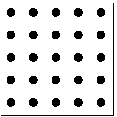
\includegraphics{Figure-01}\\
{\small basis partition corresponding to $\mathbf{r}=(0,0,0,0,0)$}
\end{center}


{\it Step $2$.} If $r_k>0$, form $r_k$ columns of length $k$ to the right
of the Durfee square. If $r_k<0$, form $|r_k|$ rows of length $k$ below
the Durfee square. The resulting partition has all successive ranks equal
to $r_k$. If $r_k=0$, then move on to $r_{k-1}$.
\begin{center}
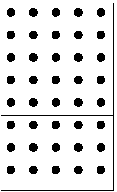
\includegraphics{Figure-02}\\
{\small $r_5=-3$, basis partition corresponding to $\mathbf{r}=(-3,-3,-3,-3,-3)$}
\end{center}


{\it Step $3$.} Next consider the difference $r_{k-1}-r_k=\delta_{k-1}$.
If this difference is $>0$, place $\delta _{k-1}$ columns of length
$k-1$ to the right of the Durfee square. If the difference is $<0$,
place $|\delta_{k-1}|$ rows of length $k-1$ below the Durfee square.
Note that all successive ranks up to the $k-1$-st are equal to
$r_{k-1}$, and the last rank is $r_k$. If $\delta_{k-1}=0$, move on to
$r_{k-2}$.
\begin{center}
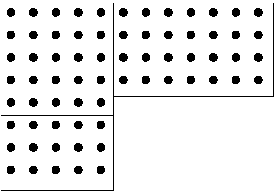
\includegraphics{Figure-03}\\
{\small $r_4 - r_5=7 = \delta_4$, basis partition corresponding to $\mathbf{r}=(4,4,4,4,-3)$}
\end{center}



{\it Step $4$ $($general$)$.} Consider the difference $r_i-r_{i+1}=\delta_i$.
If this difference is $>0$, place $\delta_i$ columns of length $i$ to the
right of the Durfee square. If the difference is $<0$, place $|\delta_i|$
rows of length $i$ below the Durfee square. If $\delta_i=0$, proceed
to $r_{i-1}$. Note that all successive ranks up to the $i$-th are equal
to $r_i$, but from then on the successive ranks are $r_{i+1}, \dots , r_k$.


{\it Step $5$.} Complete the construction by considering the final case
$i=1$ in Step~4. We end up with a basis partition with successive rank
vector $(r_1, r_2, \dots , r_k)$ as desired.
\begin{center}
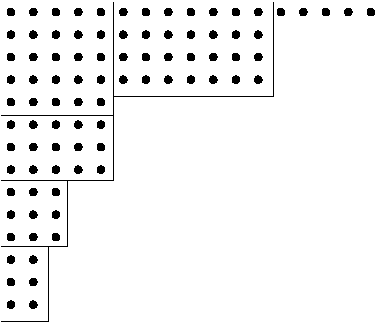
\includegraphics{Figure-04}\\
{\small $\delta_1=5$, $\delta_2=-3$, $\delta_3=-3$, $\delta_4=7$, $\delta_5=-3$, basis partition corresponding to $\mathbf{r}=(3,-2,1,4,-3)$}
\end{center}


\section{The signature of basis partitions and a theta series}\label{section5}

The combinatorial proof given in Section~\ref{section3}, and the construction of
the basis partition corresponding to successive rank vector given in
Section~\ref{section4}, lead to the definition of the {\it signature}~$\Sigma(\pi)$
of a basis partition to be the number of differences $r_i-r_{i+1}=\delta_i$
that are negative. Note that
\begin{equation*}
\Sigma (\pi)=\nu_d(\pi_b),%\label{eq:5.1}
\end{equation*}
where $\nu_d(\pi_b)$ is the number of different parts of $\pi_b$. The
combinatorial constructions of Sections~\ref{section3} and~\ref{section4} enable us to keep track
of this signature and obtain a refined generating function of basis
partitions. More precisely, if $b(n,k,s)$ denotes the number of basis
partitions of $n$ with a~${k\times k}$ Durfee square and with signature
$s$, then for a fixed $k$, we get the following refinement of~\eqref{eq:2.3}:
\begin{equation}
\sum_{n,s}b(n,k,s)q^nz^s=\frac{q^{k^2}(1+zq)\bigl(1+zq^2\bigr)\cdots \bigl(1+zq^k\bigr)}
{(1-q)\bigl(1-q^2\bigr)\cdots \bigl(1-q^k\bigr)}.\label{eq:5.2}
\end{equation}
Observe that $z=-1$ makes the right hand side of~\eqref{eq:5.2} collapse to
$q^{k^2}$. Thus, we get the partial theta series identity
\begin{equation*}
\sum_{n,k,s}b(n,k,s)q^n(-1)^s=\sum^{\infty}_{k=0}q^{k^2}.%\label{eq:5.3}
\end{equation*}
This has the following partition interpretation.

\begin{Theorem}\label{thm:3}
For an integer $n$, consider the difference between
the number of basis partitions of n with even signature and the number of
basis partitions with odd signature. This difference is $1$ if n is
a perfect square, and $0$ otherwise.
\end{Theorem}

Actually, the discussion of the signature leads to a refinement of
Theorems~\ref{thm:1} and~\ref{thm:2}, where the weight $2^t$ is replaced by $(1+z)^t$ so
that Theorems~\ref{thm:1} and~\ref{thm:2} correspond to the case $z=1$ and Theorem~\ref{thm:3}
follows as the special case $z=-1$. We state these refinements as
Theorem~\ref{thm:4}\,(i) and~(ii) below.

\begin{Theorem}\label{thm:4}\quad
\begin{enumerate}\itemsep=0pt
\item[$(i)$]
Let $\mathbf{R}$ denote the set of Rogers--Ramanujan partitions. For
each partition $\pi\in \mathbf{R}$,
\begin{equation}
\pi\colon\ b_1+b_2+\dots +b_k, \qquad b_i-b_{i+1}\ge 2 \quad \text{for} \
i=1,2,\dots , k-1, \ \text{and} \ b_k\ge 1,\label{eq:5.4}
\end{equation}
let its weight be $\omega_z(\pi)=(1+z)^t$, where $t$ is the number of strict inequalities in~\eqref{eq:5.4}. Then for each $n$ and $k$ we have
\[
\sum_sb(n,k,s)z^s=\sum_{\pi\in \mathbf{R},\, \sigma(\pi)=n,\, \nu(\pi)=k}\omega_z(\pi).
\]
\item[$(ii)$]
Let $\mathbf{P}$ denote the set of primary partitions. For
each partition $\pi\in \mathbf{P}$,
\begin{equation}
\pi\colon b_1+b_2+\dots +b_k, \qquad b_i-b_{i+1}\ge 0 \quad \text{for} \
i=1,2,\dots , k-1, \ \text{and} \ b_k\ge k, \label{eq:5.5}
\end{equation}
let its weight be $\omega_z(\pi)=(1+z)^t$, where $t$ is the
number of strict inequalities in~\eqref{eq:5.5}. Then for each $n$ and $k$ we have
\[
\sum_sb(n,k,s)z^s=\sum_{\pi\in \mathbf{P},\, \sigma(\pi)=n,\, \nu(\pi)=k}\omega_z(\pi).
\]
\end{enumerate}
\end{Theorem}

\section{A Franklin type involution for Theorem~\ref{thm:3}}\label{section6}

For Euler's celebrated pentagonal number theorem, Fabian Franklin provided
an elegant combinatorial proof (see~\cite{An-book}). Franklin's proof utilized an
involution on Ferrers graphs of partitions of an integer into distinct
parts by considering the {\it base} and {\it slope} on these graphs.
We will now produce an involution on the Ferrers graphs of basis partitions,
in which the base and slope are replaced by {\it bottom block} and
{\it right block}.

Given a Ferrers graph of a basis partition, we define a {\it block} to be
the full collection of columns of a given length to the right of
the Durfee square, or the full collection of rows of a given length
below the Durfee square. Thus, the part to the right of the Durfee
square is a collection of blocks, as is the portion below the Durfee
square. The number of blocks below the Durfee square is equal to the
number of different parts below the Durfee square, and therefore equal
to the signature of the basis partition.

Next we define the length of a block to be its column length if it is
to the right of the Durfee square, and its row length if it is below
the Durfee square. Since a basis partition $\pi$ is characterized by the
property that no column of $\pi_r$ equals a row of $\pi_b$, this is
equivalent to saying that the blocks in the graph of a basis partition
all have different lengths.

Finally, define the {\it right block} to be the block on the extreme
right in $\pi_r$, and the {\it bottom block} to be the block at the
very bottom of~$\pi_b$. Note that the lengths of the right block and
the bottom block (if they exist) are different. This leads us to the following definitions.

{\bf Definition B.} Given the Ferrers graph of a basis partition, we call
it a Type~B partition, if the bottom block exists, and if its length is
less than the length of the right block (if the right block exists).
If the right block does not exist, but the bottom block does, it is
still a Type B partition.

{\bf Definition~R.} Given the Ferrers graph of a basis partition, we call
it a Type R partition, if the right block exists, and if its length is
less than the length of the bottom block (if the bottom block exists).
If the bottom block does not exist, but the right block does, it is
still a Type R partition.

Thus, every Ferrers graph of a basis partition, unless it is just the
Durfee square, is either a~Type~B partition or a~Type~R partition, but
not both.

{\bf Involution.} Now we define a mapping as follows. If we have
a~Type~B partition,
we move the bottom block, convert its rows into columns, and place it
on the extreme right thereby making it the (new) right block. Thus, we
create a Type R partition. Conversely, if we have a~Type~R partition,
we move the right block, convert its columns into rows, and place it
at the very bottom of the graph to create a Type B partition. Notice
that under this mapping, the {\it parity} of the number of parts below
the Durfee square, namely the {\it parity of the signature}, changes. The
only graph on which this mapping does not apply, is the graph consisting
of just the Durfee square and so this provides a combinatorial proof of
Theorem~\ref{thm:3}.

{\bf Conjugation as an involution.} It is worth noting that if $\pi$ is
a basis partition, then its (Ferrers) conjugate $\pi^*$is also a basis
partition. This is because basis partitions $\pi$ are characterized by
the property that no row of $\pi_b$ equals a column of $\pi_r$, and this
property is preserved under conjugation. Also, this characterization
implies that $\pi$ and $\pi^*$ are different basis partitions unless
the graph of $\pi$ is simply a Durfee square. Thus, by matching every basis
basis partition~$\pi$ with its conjugate $\pi^*$, we see the number
$b(n)$ of basis partitions of $n$ is even unless $n$ is a~perfect square.
This parity property of $b(n)$ follows from Theorem~\ref{thm:3} but conjugation
as an involution does not prove Theorem~\ref{thm:3}.

\section{Basis partitions with a prescribed signature}\label{section7}

In this section, we study the generating function of basis partitions
with a prescribed signature, and discuss how they are connected to
the Rogers--Ramanujan partitions. We will use the standard notation
\[
(a;q)_n=(a)_n=\prod^{n-1}_{j=0}\bigl(1-aq^j\bigr),
\]
for any complex number $a$ and a non-negative integer $n$, and when $|q|<1$
\[
(a)_{\infty}=\lim_{n\to\infty}(a)_n=\prod^{\infty}_{j=0}\bigl(1-aq^j\bigr).
\]

The construction in Section~\ref{section3} showed that we get basis partitions
from primary partitions (equivalent to Rogers--Ramanujan partitions)
by sliding blocks from the right of the Durfee square and placing them
below the Durfee square after converting the columns of these blocks
into rows. If there are $t$ blocks in the portion $\pi_r$, and $j$ of
these have to be moved, then the number of choices is
$\left(\begin{smallmatrix} t\\ j\end{smallmatrix}\right)$.
Thus, from this observation, and by collecting the coefficient of $z^j$
in Theorem~\ref{thm:4}, we get the following refinement of Hirschhorn's theorem.

\begin{Theorem}\label{thm:5}
Let $\mathbf{R}$ denote the set of Rogers--Ramanujan partitions.
Suppose a partition~${\pi\!\in\! \mathbf{R}}$,
\begin{equation*}
\pi\colon\ b_1+b_2+\dots +b_k, \qquad b_i-b_{i+1}\ge 2 \quad \text{for} \
i=1,2,\dots , k-1, \ \text{and} \ b_k\ge 1,%\label{eq:7.1 }
\end{equation*}
has $t$ strict inequalities in~\eqref{eq:5.4}. For a given $j$, define the weight
\[
\omega_j(\pi)=\bin{t}{j}.
\]
Then for each $n$ and $k$, we have
\[
b(n,k,j)=\sum_{\pi\in \mathbf{R},\, \sigma(\pi)=n,\, \nu(\pi)=k}\omega_j(\pi).
\]
\end{Theorem}

Theorem~\ref{thm:5} is what we get combinatorially by looking at the sliding
of blocks. But we get a~{\it different} connection between
basis partitions of a prescribed signature and Rogers--Ramanujan partitions
by evaluating the coefficient of~$z^j$ in~\eqref{eq:5.2}.

Denote by $B(n;j)$ the number of basis partitions of $n$ with signature
$j$ (note the difference with $b(n;k)$). Thus
\begin{equation}
\sum^{\infty}_{k=0}\frac{q^{k^2}(-zq)_k}{(q)_k}=
\sum_j z^j\sum_nB(n;j)q^n.\label{eq:7.1}
\end{equation}
But then
\begin{align}
\sum^{\infty}_{k=0}\frac{q^{k^2}(-zq)_k}{(q)_k}& =
\sum^{\infty}_{k=0}\frac{q^{k^2}}{(q)_k}\sum^k_{j=0}z^jq^{j(j+1)/2}
\qbin{k}{j}
\nonumber\\
& =\sum^{\infty}_{j=0}\frac{z^jq^{(j(j+1)/2}}{(q)_j}
\sum^{\infty}_{i=0}\frac{q^{(i+j)^2}}{(q)_i}=
\sum^{\infty}_{j=0}\frac{z^jq^{(3j^2+j)/2}}{(q)_j}
\sum^{\infty}_{i=0}\frac{q^{i^2+2ij}}{(q)_i}.\label{eq:7.2}
\end{align}
By comparing coefficients of $z^j$ in~\eqref{eq:7.1} and~\eqref{eq:7.2}, we get the
generating function of basis partitions with a prescribed signature as
\begin{equation*}
\sum^{\infty}_{n=0}B(n;j)q^n=
\frac{q^{(3j^2+j)/2}}{(q)_j}
\sum^{\infty}_{i=0}\frac{q^{i^2+2ij}}{(q)_i}.%\label{eq:7.3}
\end{equation*}
We will now interpret this combinatorially.

The term
\smash{${q^{(3j^2+j)/2}}/{(q)_j}$}
is the generating function of partitions into $j$ parts with difference
$\ge 3$ between the parts and smallest part $\ge 2$. The term
\smash{${q^{i^2+2ij}}/{(q)_i}$}
is the generating function for partitions into $i$ parts with difference
$\ge 2$ between the parts (namely, the Rogers--Ramanujan partitions), but
with the condition that the smallest part is~${\ge 2j+1}$. Thus, we have
the following result.

\begin{Theorem}%\label{thm:6}
The number of basis partitions $B(n;j)$ of an integer $n$ with signature $j$ is equal to the number of vector partitions
$(\pi_3,\pi_2)$ of $n$, where $\pi_3$ is a partition into $j$ parts
differing by~$\ge 3$ and least part $\ge 2$, and $\pi_2$
is a partition into parts differing by~$\ge 2$ and least part~${\ge 2j+1}$.
\end{Theorem}

It is possible to convert these vector partitions into ordinary partitions,
but then we need to count the resulting Rogers--Ramanujan partitions with
weights. This is complicated and so we do not pursue it here.

\section{Complete basis partitions}

One of the fundamental properties of partitions into distinct parts is that
if they are represented as Ferrers graphs, then the conjugate partitions have
the property that every integer from~1 up to largest part occurs as a part.
Motivated by this characterization of partitions into distinct parts, we now
define a {\it complete basis partition} $\pi$ to be a basis partition
with the property that if $|D(\pi)|=k$, then every integer $j$ from 1 to $k-1$
occurs either as a row length below $D(\pi)$ or as a~column length to the
right of $D(\pi)$, but not both because $\pi$ is a basis partition ($D(\pi)$ is Durfee square of~$\pi$). The reason
for requiring only row (column) lengths up to $k-1$ will become clear below.
From the
construction of basis partitions in Section~\ref{section4}, it follows that the an integer~$j$
between~1 and $|D(\pi)|$ is missed as either a row length below $D(\pi)$
or a column length to the right of $D(\pi)$ if and only if in the successive
rank vector $\mathbf{r}=(r_1,r_2,\dots ,r_k)$, we have $r_j=r_{j+1}$, where we
formally set $r_{k+1}=0$. Thus, we have the following characterization of
complete basis partitions.

{\bf Characterization.} A basis partition with a $k\times k$
Durfee square is complete if and only if its successive rank vector
$\mathbf{r}=(r_1,r_2,\dots ,r_k)$ has the property that
\begin{equation*}
r_j\ne r_{j+1} \qquad \text{for} \ j=1,2,\dots ,k-1.%\label{eq:8.1}
\end{equation*}

We note that a row (column) of length~$k$ is missing precisely when $r_k=0$.

We will now compute the generating function of complete basis partitions by
connecting them with partitions into distinct parts. For this, we consider
partitions into distinct parts which are primary, that is in their Ferrers
graph representation, there is nothing below the Durfee square. So let $\pi$
be a primary partition into distinct parts with $|D(\pi)|=k$. This Ferrers
graph has two properties:
\begin{enumerate}\itemsep=0pt
\item[(i)] To the right of the Durfee square there is a right-angled
isosceles triangle of nodes with the two equal sides of the triangle being
of length $\ge k-1$. This guarantees that there are at least $\bigl(3k^2-k\bigr)/2$ nodes
in the Ferrers graph.
\item[(ii)] Every integer between 1 and $k-1$ occurs as a column length to the right
of $D(\pi)$.
\end{enumerate}

In~\cite{Al0097}, we discussed the construction of all partitions into distinct parts
from primary partitions into distinct parts by means of the sliding operation.
In doing so we noted in~\cite{Al0097} that at most one column of a given length could be
slid down because the resulting partition has to have distinct parts.
Here we shall focus of generating all complete basis partitions from primary
partitions. What this means is that once we slide a column of a certain length
$j$ to the right of the Durfee square, we have to slide all columns of length
$j$. Thus, for a column of length~$j$ on the right, there are precisely two
choices -- to slide the entire set of such columns or not to slide at all. Since
these choices are independent, and every integer $j$ from 1 to $k-1$ occurs as
a~column length, each primary partition into distinct parts generates at least
$2^{k-1}$ complete basis partitions. If~the graph of $\pi$ has a column of
length $k$, this will provide two more independent choices. Thus, if~$b_c(n)$
denotes the number of complete basis partitions of~$n$, its generating
function is
\begin{equation}
\sum^{\infty}_{n=0}b_c(n)q^n=
1+\sum^{\infty}_{k=1}\frac{2^{k-1}q^{(3k^2-k)/2}\bigl(1+q^k\bigr)}{\bigl(1-q^k\bigr)}.\label{eq:8.2}
\end{equation}

The sliding operation that yielded the complete basis partitions from primary
basis partitions shows that we could count complete basis partitions
by keeping track of their signature. More precisely, if $b_c(n;j)$ denotes
the number of complete basis partitions with signature $j$, then
\begin{equation}
\sum^{\infty}_{n=0}\sum^{\infty}_{j=0}b_c(n;j)z^jq^n=
1+\sum^{\infty}_{k=1}\frac{(1+z)^{k-1}q^{(3k^2-k)/2}\bigl(1+zq^k\bigr)}{\bigl(1-q^k\bigr)}.\label{eq:8.3}
\end{equation}
Notice that when $z=-1$, the series in~\eqref{eq:8.3} reduces to $1+q$. Thus, we have the following.

\begin{Theorem}\label{thm:7}
For each integer $n\ge 2$, the number of
complete basis partitions of even signature is equal to the number of
complete basis partitions of odd signature. In particular, for $n\ge 2$, $b_c(n)$~is always even.
\end{Theorem}

Theorem~\ref{thm:7} can also be proved using the Franklin type involution discussed in
Section~\ref{section6}.

The hook lengths of primary partitions into distinct parts yield partitions
into parts that differ by at least~3, and conversely every partition
$\tilde\pi$ into parts that differ by at least 3 can be realized in terms of
hooks of a primary partition~$\pi$ into distinct parts. If $|D(\pi)|=k$,
then $\tilde\pi$ has exactly~$k$ parts. With this identification, we have the following.

\begin{Theorem}\label{thm:8}
Let $D_3$ denote the set of partitions whose
parts differ by at least $3$. For a~partition~$\tilde\pi\in D_3$, let
its weight be $w(\tilde\pi)=2^{\nu(\tilde\pi) -1}$
if $\tilde\pi$ has $1$ as a part, and
${w(\tilde\pi)=2^{\nu(\tilde\pi)}}$ otherwise, where $\nu(\tilde\pi)$
{{is the number of parts of}} $\tilde\pi$. Then
\[
b_c(n)=\sum_{\tilde\pi\in D_3, \sigma(\tilde\pi)=n}w(\tilde\pi).
\]
\end{Theorem}

Theorem~\ref{thm:8} is the combinatorial interpretation of~\eqref{eq:8.2}.

\begin{Remark*}
Using~\eqref{eq:8.2} or Theorem~\ref{thm:8}, one can show that
$b_c(n)\equiv 0 \pmod 4$ for $n\ge 5$.
More generally, using~\eqref{eq:8.2} or Theorem~\ref{thm:8} one can study the values of $n$ for
which $b_c(n)$ is a~multiple of $2^k$.
\end{Remark*}

\section[Basis partitions among partitions with non-repeating odd parts]{Basis partitions among partitions\\ with non-repeating odd parts}\label{section9}


We conclude the paper with a study of basis partitions among the set $P_{\rm o,d}$
of partitions with non-repeating odd parts. There are similarities with the
theory of basis partitions for unrestricted partitions, but there are very
interesting differences, and the results quite elegant. That is what motivated
this study.

Partitions with non-repeating even parts have been studied extensively owing
to the famous Lebesgue identity. Comparatively less is known about partitions
with non-repeating odd parts. Our interest in partitions with non-repeating
odd parts is due to the fact that if they are represented in terms of 2-modular
Ferrers graphs (that is Ferrers graphs in which there is a 2 at every node
except possibly at the last node on the right which would be 1 if the part
is odd), then the ones can occur only in the corners. Also the conjugate of
such a graph will also be a~2-modular graph of a partition with non-repeating
odd parts. By exploiting these properties, we established in~\cite{Al2010} a Lebesgue
type expansion for the two parameter generating function
\[
\prod^{\infty}_{m=1}\frac{\bigl(1+bzq^{2m-1}\bigr)}{\bigl(1-zq^{2m}\bigr)}
\]
of partitions with non-repeating odd parts and studied connections between this
Lebesgue type identity and various fundamental $q$-hypergeometric identities.
More recently in~\cite{Al2016}, we studied the combinatorial properties of partitions in
$P_{\rm o,d}$ by means of this 2-modular representation. The results in~\cite{Al2010} and~\cite{Al2016}
constitute the first systematic study of partitions in $P_{\rm o,d}$ by means of
their 2-modular graphs. In this section, we will study {\it minimal basis partitions}
and {\it basis partitions} among
the members of $P_{\rm o,d}$. Results on such partitions in $P_{\rm o,d}$ were reported
in~\cite{Al2016}, but here we discuss these two types of partitions in~$P_{\rm o,d}$ in greater detail, and also provide a combinatorial method to construct them. Indeed, in~\cite{Al2016}, reference is made to this paper for details and the combinatorial construction given below.

{\it From now, on by a partition we mean one in $P_{\rm o,d}$ and by a Ferrers graph, we mean a $2$-modular Ferrers graph. We shall from now on refer to the Ferrers graph of unrestricted partitions as ordinary Ferrers graphs.}

Given a 2-modular Ferrers graph of a partition $\pi\in P_{\rm o,d}$, we define
the {\it length} of a row (column) to be the number of nodes in it, and the
{\it size} of a row (column) to be the sum of the nodes in it. Thus, the
row $2$, $2$, $1$ will have length $3$ and size $5$. We do not need this distinction
for ordinary Ferrers graphs.
Next if $\pi\in P_{\rm o,d}$ has a $k\times k$ Durfee square $D(\pi)$ in its
2-modular graph, we define its successive rank vector to be
$\mathbf{r}=(r_1,r_2,\dots ,r_k)$, where
$
r_j= \text{\it size of the $j$-th row} - \text{\it size of the $j$-th column}$.
By a {\it minimal basis partition}, we mean a~partition $\mu\in P_{\rm o,d}$ for
which the sum of its parts $\sigma(\mu)$ is minimal with respect to a given
successive rank vector. We will now establish the following statement.

\begin{Theorem}\label{thm:9}
Given any vector of integers
$\mathbf{r}=(r_1,r_2,\dots ,r_k)$, there exists a unique minimal basis
partition $\mu$ for which $\mathbf{r}$ is the successive
rank vector.
\end{Theorem}

We will establish Theorem~\ref{thm:9} by actually constructing $\mu$ from a given
$\mathbf{r}$.
Before proceeding with the construction, we note that the Durfee square
$D(\pi)$ of any partition~${\pi\in P_{\rm o,d}}$ will have all entries as twos,
except possibly at the right hand bottom corner where there could be a 1.
If there is a 1 in the Durfee square, then in the graph there will be no nodes
to its right in the same row and no nodes below it in the same column.

We will illustrate the construction of $\mu$ in a sequence of steps with the
successive rank vector $\mu=(1,-4,1,2,-5)$, but the construction applies in
general as in Section~\ref{section4}. The construction, although similar to that in
Section~\ref{section4} has an important differences involving parity which we will point
out below. That is why we give this construction even though there is overlap
with Section~\ref{section4}.



{\bf Construction of the minimal basis partition.}
Let the given successive rank vector be~${\mathbf{r}=(r_1,r_2,\dots ,r_k)}$.


{\it Step $1$.} Form a $k\times k$ Durfee square with a 1 at the bottom right
node and twos everywhere else. This is the minimal basis partition
corresponding to the vector
\begin{center}\samepage
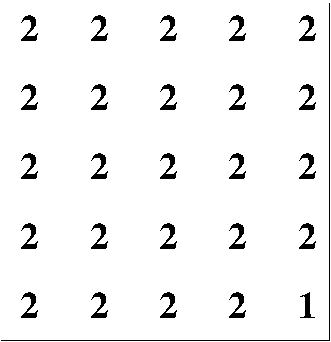
\includegraphics[scale=0.45]{Figure-05}\\
{\small $\mathbf{r}=(0,0,0,0,0)$}
\end{center}
\pagebreak

{\it Step $2$.} If $r_k=0$, retain the 1 in the Durfee square and move to
$r_{k-1}$. If $r_k>0$ (resp.~$<0$), change the 1 to a 2 in the Durfee square,
and represent $r_k$ (resp.\ $|r_k|$) in 2-modular form as a~row (resp.\ column)
to the right of (resp.\ below) the k-th row of the Durfee square. Fill every
thing above (resp.\ to the left of) the newly formed row (resp.\ column)
with twos. The resulting partition will have the $k$-th successive rank
as $r_k$, and all other successive ranks will be equal to $r_k$ if $r_k$ is
even; if $r_k$ is odd, then since the end of the $k$-th row (resp.\ column)
will have a~1 with twos elsewhere, all other successive ranks will be $r_k+1$
if $r_k>0$ or $r_k-1$ if~${r_k<0}$. The important thing is that we now have $r_k$
as the $k$-th successive rank. We will represent this new vector as
$\bigl(r^*_{k}, r^*_k,\dots ,r^*_k, r_k\bigr)$. This is an important difference between
the situation here and what we had in Section~\ref{section4}. In our example, we have
constructed the minimal basis partition corresponding to
\begin{center}
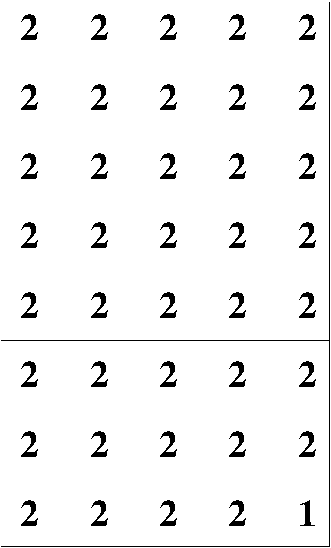
\includegraphics[scale=0.45]{Figure-06}\\
{\small $\mathbf{r}=(-6,-6,-6,-6,-5)$}
\end{center}

{\it Step $3$.} Next consider the difference $r_{k-1}-r^*_k=\delta_{k-1}$. If this
difference is $>0$, write $\delta_{k-1}$ in 2-modular form to the right of the
$(k-1)$-st row and fill everything above that with twos. If $\delta_{k-1}<0$,
write $|\delta_{k-1}|$ in 2-modular form as a column below the
$(k-1)$-st column
and fill everything to its left with twos. If $\delta_{k-1}=0$, move on to
$r_{k-2}$. Thus, we have formed the minimal basis partition who last two
successive ranks are $r_{k-1}$ and $r_k$. The remaining successive ranks
will all be
equal, their values being $r_{k-1}$ if it is even, or $r_{k-1}+1$ if $r_{k-1}>0$
and odd, or $r_{k-1}-1$ if $r_{k-1}<0$ and odd. We represent these remaining
successive ranks by $r^*_{k-1}$. Thus, we have the minimal basis partition
corresponding to $\bigl(r^*_{k-1},r^*_{k-1},\dots ,r^*_{k-1}, r_{k-1},r_k\bigr)$. In our example,
we have formed the minimal basis partition corresponding to
\begin{center}
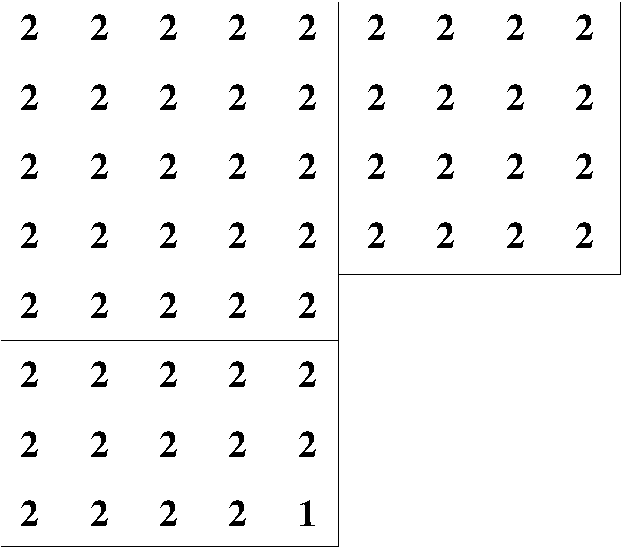
\includegraphics[scale=0.45]{Figure-07}\\
{\small $\mathbf{r}=(2,2,2,2,-5)$}
\end{center}


{\it Step $4$ $($general$)$.} Consider the difference $r_j-r^*_{j+1}=\delta_j$.
If this difference is $>0$, represent~$\delta_j$ in 2-modular form as a row
to the right of the $j$-th row, and fill everything above with twos. If the
difference is $<0$, represent $|\delta_j|$ in 2-modular form as a column
below the $j$-th column, and fill everything to its left with twos.
If $\delta_j=0$, proceed to $r_{j-1}$. Note that all successive ranks from
$r_j$ on are $r_j,r_{j+1},\dots , r_k$. the remaining $j-1$ successive ranks are
all equal and we represent them by $r^*_j$. So we have formed the minimal
basis partition corresponding to~$\bigl(r^*_j,r^*_j,\dots ,r^*_j,r_j,r_{j+1},\dots ,r_k\bigr)$.

{\it Step $5$.} Complete the construction by considering the final case $j=1$
in Step~4. we then have the minimal basis partition $\mu$ corresponding to the
given successive rank vector $\mathbf{r}$. In our example, we have the minimal
basis partition corresponding to
\begin{center}
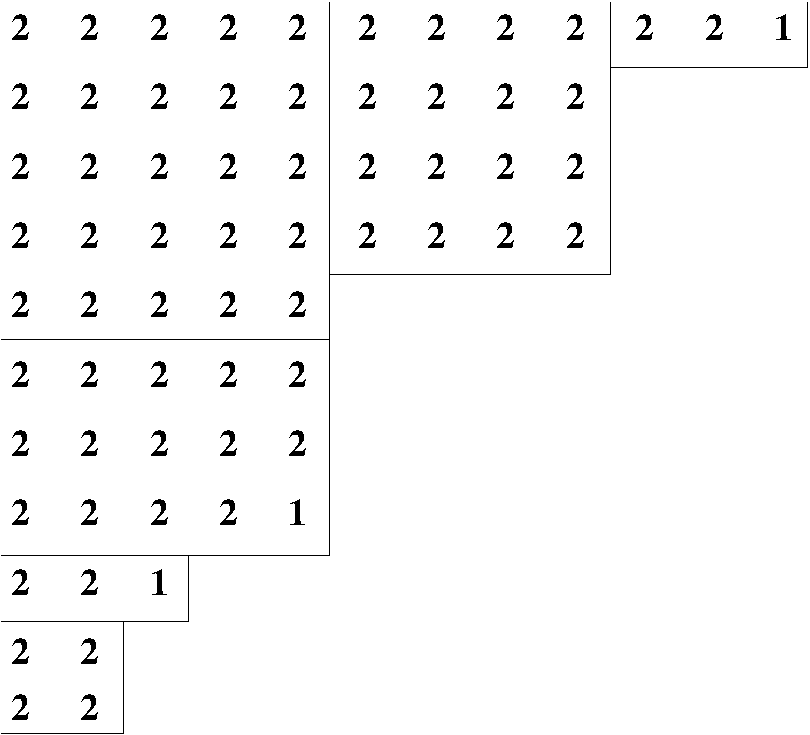
\includegraphics[scale=0.45]{Figure-08}\\
{\small $\mathbf{r}=(1,-4,1,2,-5)$}
\end{center}

Our construction has shown that minimal basis partitions are
characterized by the following.

\begin{Theorem}%\label{thm:10}
The partition $\mu$ is a minimal basis partition if and only if
no row below the Durfee square is equal in length
to a column to the right of the Durfee square, and the right hand
bottom entry in the Durfee square is~$1$ if the last successive rank is~$0$.
\end{Theorem}

\begin{Remark}\quad
\begin{enumerate}\itemsep=0pt
\item[$(1)$] It is very interesting that even though minimal basis
partitions were defined in terms of {\it size}, the characterization is
in terms of {\it length}. In view of this, we now define a
{\it basis partition} to be a partition in $P_{o.d}$ for which no row
below the Durfee square is equal \textit{in size} to a column to the right of
the Durfee square. For example, in a basis partition we could have
$2$, $2$, $1$ as a row and $2$, $2$, $2$ as a column, but this is not permissible in a minimal
basis partition. Thus, every minimal basis partition is a basis partition, but
the converse is not true.\looseness=-1

\item[$(2)$] Berkovich and Garvan~\cite{Be-Ga02} have studied successive ranks among members of $P_{\rm o,d}$, but they defined the rank as the difference between the lengths of the row and the column, not in terms of the differences in sizes as we have considered here. But Berkovich--Garvan did not study basis partitions with their definition.
\end{enumerate}
\end{Remark}


{\bf Construction of basis partitions from minimal basis
partitions.}
The set of all basis partitions can be constructed from the set of all
minimal basis partitions as we show now.

Suppose we are given a minimal basis partition $\mu$. If the last successive
rank is 0, then in the Durfee square of $\mu$ we have a 1. If we replace
this 1 by a 2, the last rank would still be 0 and so we would get a basis
partition corresponding to the same successive rank vector.

Note that in any hook of $\mu$, there can be at most one 1 -- either at the
northeastern end or at the southwestern end but not both. Also, if there is
a 1 in a hook of $\mu$, then the 2 at the other end cannot be a corner, because
it is were, then $\mu$ would have a row and column of equal length. So if
there is a 1 in a hook of $\mu$, we could replace that by a 2, and add a 1
to the other end of the hook {\it provided} there is a 2 immediately
to the left of (or above) the position where are introducing the new 1. We call
such a hook as an allowable hook. If a minimal basis partition has $\alpha$
allowable hooks (including the special case where the Durfee square has a 1
in it), then with each such hook we have the choice of making such a change
or not. Thus, each minimal basis partition with $\alpha$ allowable hooks, will
spawn $2^{\alpha}$ basis partitions, including $\mu$, all with the same
successive rank vector. This procedure will generate all basis
partitions from minimal basis partitions.

{\bf Constructing basis partitions by the sliding operation.}
There is a nice way to get all basis partitions from primary partitions in
$P_{\rm o,d}$ using the sliding operation.

In $P_{\rm o,d}$ we define a primary partition to be one such that in its 2-modular
Ferrers graph there are no nodes below the Durfee square. In~\cite{Al2016} the
construction of all partitions in $P_{\rm o,d}$ from primary partitions is
discussed. This involves the sliding operation along with the creation of
secondary partitions generated by primary partitions. For the purpose
of constructing basis partitions, only primary partitions and the sliding
operation are needed and we discuss this now.

Given a primary partition, we consider a column on length $j$ only of twos
to the right of the Durfee square.
If there are several such columns of the same length~$j$, we either can slide
all the columns or none, thereby giving us two choices for each collection
of columns of twos of a~given length. If we have a column of length~$j$ but
whose
size is odd, then such a column can also be slid down giving us once again
two choices. Through such sliding operations, all basis partitions can be
generated. Since the weights now will be powers of~2, there is an analogue to
Hirschhorn's Theorem~\ref{thm:1},
but to determine these weights we need to consider separately columns
having only twos, and columns of twos ending in a one.
But before stating this, we will
consider the hook operation on primary partitions.

Given a primary partition in $P_{\rm o,d}$, consider the partition $\tilde\pi$
generated by summing the entries on the hooks of $\pi$. This will be a
partition whose parts will differ by $\ge 4$ with strict inequality if a part
is odd. We call such partitions as {\it special},
and denote the set of all special partitions by $\Psi$.
Conversely given a special
partition, we can find a primary partition whose hook lengths will correspond
to the given special partition. Thus, the hook operation
\begin{equation}
\pi\mapsto \tilde\pi\label{eq:9.2}
\end{equation}
is a bijection between primary partitions and special partitions. It is to be
noted that the existence of a column of length $j$ to the right of the Durfee
square of a primary partition~$\pi$ is equivalent to saying
that the difference between the $j$-th part and the $(j+1)$-st part
of~$\tilde\pi$ is~${>4}$. Here we adopt the convention that if $\tilde\pi\colon
b_1+b_2+\dots +b_k$, then $b_{k+1}=-2$.
The construction of basis partitions from primary partitions in the preceding
paragraph together with~\eqref{eq:9.2} yields the following analogue to
Hirschhorn's theorem:

\begin{Theorem}
%\label{thm:11}
If $\tilde\pi\colon b_1+b_2+\dots+ b_k$ is a special partition, then let
\[
b_i - b_{i+1} \ge m(b_{i+1}) := 4 + [b_{i+1}]_2,
\]
where $[n]_2=0$ if $n$ is even, and $[n]_2=1$ if $n$ is odd.
Define the weight $w(\tilde\pi)=2^\ell$, where
\begin{align*}
\ell &= \{\mbox{number of gaps $ b_i - b_{i+1} > m(b_{i+1})$}\} \\
& \quad{}+
\{\mbox{number of gaps $ b_i - b_{i+1} > m(b_{i+1})+2$ when $b_i$ is odd}\},
\end{align*}
with the convention $b_{k+1}=-2$.
If $b(n)$ is the number of basis partitions of
n in $P_{\rm o,d}$, then
\begin{equation*}
b(n)=\sum_{\tilde\pi\in \Psi,\,\sigma(\tilde\pi)=n} w(\tilde\pi).%\label{eq:9.3}
\end{equation*}
More generally, if $b(n,j)$ is the number of basis partitions in
$P_{\rm o,d}$ {{with signature j, then}}
\begin{equation*}
\sum_jb(n;j)z^j=\sum_{\tilde\pi\in \Psi,\, \sigma(\tilde\pi)=n}w_z(\tilde\pi),%\label{eq:9.4}
\end{equation*}
where $w_z(\tilde\pi)=(1+z)^{\ell}$, if $\tilde\pi$ with $\ell$
as above.
\end{Theorem}



{\bf The generating function of basis partitions and minimal basis
partitions.}
We will begin with the generating function of basis partitions which is
easier to derive.

To get the generating function of basis partitions,
we start with a $k\times k$ Durfee square of all twos which we call Case 2,
and a $k\times k$ Durfee square of twos with a 1 at the bottom right hand
corner, which we call Case 1. For Case 2, consider a collection of integers
all equal to~$2j$ represented as a row of twos~$j$ in number,
where $1\le j\le k$. We have
either a choice of placing all of them to the right of the Durfee square as
columns, or all of them as rows below the Durfee square. This gives two choices
for each set of such $2j$. Similarly, if we have an integer~${2j-1}$ occurring
singly, we could either place represent it as a column to the right of the
Durfee square or as a row below the Durfee square. This yields the generating
function
\begin{equation}
q^{2k^2}\frac{\bigl(-q^2;q^2\bigr)_k}{\bigl(q^2;q^2\bigr)_k} \bigl(-2q;q^2\bigr)_k.\label{eq:9.5}
\end{equation}
For Case 1 with a $k\times k$ Durfee square, the argument is the same as above
except that we can only have $1\le j\le k-1$, since $j=k$ is not allowed. This
yields the generating function
\begin{equation}
q^{2k^2-1}\frac{\bigl(-q^2;q^2\bigr)_{k-1}}{\bigl(q^2;q^2\bigr)_{k-1}} \bigl(-2q;q^2\bigr)_{k-1}.\label{eq:9.6}
\end{equation}
To get the generating function of $b(n)$, the number of basis partitions of
$n$, we need to sum the expressions in~\eqref{eq:9.5} and~\eqref{eq:9.6} over all $k$ to get
\begin{equation}
\sum^{\infty}_{n=0}b(n)q^n=
\sum^{\infty}_{k=0}\frac{q^{2k^2}\bigl(-q^2;q^2\bigr)_k\bigl(-2q;q^2\bigr)_k}{\bigl(q^2;q^2\bigr)_k}
+\sum^{\infty}_{k=1}\frac{q^{2k^2-1}\bigl(-q^2;q^2\bigr)_{k-1}\bigl(-2q;q^2\bigr)_{k-1}}{\bigl(q^2;q^2\bigr)_{k-1}}.
\label{eq:9.7}
\end{equation}

The above combinatorial derivation of the generating function actually allows
us to refine~\eqref{eq:9.7} by introducing parameters $z$ and $b$ whose powers keep
track of the signature and the number of odd parts of the partition,
respectively. That is if $b(n;j,i)$ denotes the number of basis partitions of
$n$ with signature $j$ and the number of odd parts equal to $i$, then~\eqref{eq:9.7}
refines to
\begin{gather}
\sum^{\infty}_{k=0}\frac{q^{2k^2}\bigl(-zq^2;q^2\bigr)_k\bigl(-b(1+z)q;q^2\bigr)_k}{\bigl(q^2;q^2\bigr)_k}
+\sum^{\infty}_{k=1}\frac{bq^{2k^2-1}\bigl(-zq^2;q^2\bigr)_{k-1}\bigl(-b(1+z)q;q^2\bigr)_{k-1}}
{\bigl(q^2;q^2\bigr)_{k-1}}
\nonumber\\
\qquad{}=\sum_{n,j,i}b(n;j,i)b^iz^jq^n.\label{eq:9.8}
\end{gather}

To determine the generating function of minimal basis partitions, we need
to observe that in Case 1, when the Durfee square has dimension $k\times k$, if a collection
of parts all equal to $2j$ are represented as a set of columns to the
right of the Durfee square or as a set of rows below the Durfee square,
but not both, then the integer $2j-1$ if it is to be included in the graph,
\textit{has to be placed alongside} the collection of $2j$. There is no choice as to
where to place the $2j-1$ if the $2j$ occurs. But then, if $2j$ \textit{does not occur},
we could have $2j-1$ represented either as a row below the Durfee square or
as a column to the right of the square, thereby giving two choices. With
regard to Case~2, the above observations in this paragraph all hold. In
addition, we need to note that the last entry in the successive rank vector
has to be non-zero, thereby forcing the graph to have either a row of
{\it length} $k$ below the Durfee square or a~column of {\it length}~$k$
to the right of the square, but not both. This row or column of length~$k$
could represent either $2k-1$ or $2k$. With these observations, we can
suitably modify~\eqref{eq:9.7} and write down the generating function of $b_m(n)$,
the number of minimal basis partitions of $n$, namely,
\begin{align}
&\sum^{\infty}_{n=0}b_m(n)q^n=1+ \sum^{\infty}_{k=1}q^{2k^2-1}\prod^{k-1}_{j=1}
\biggl\{1+2q^{2j-1}+\frac{2q^{2j}\bigl(1+q^{2j-1}\bigr)}{\bigl(1-q^{2j}\bigr)}\biggr\}
\nonumber\\
&\qquad{}+ \sum^{\infty}_{k=1}q^{2k^2}\prod^{k-1}_{j=1}
\biggl\{1+2q^{2j-1}+\frac{2q^{2j}\bigl(1+q^{2j-1}\bigr)}{\bigl(1-q^{2j}\bigr)}\biggr\}
\times
\biggl(2q^{2k-1}+\frac{2q^{2k}\bigl(1+q^{2k-1}\bigr)}{\bigl(1-q^{2k}\bigr)}\biggr).\label{eq:9.9}
\end{align}

As in the case of the generating function of basis partitions, we can refine
\eqref{eq:9.9}, but here it is best to keep track of the number of different lengths
below the Durfee square, which we call as $\ell$-{\it signature}, which,
for the sake of clarity, we will keep track by a parameter $\zeta$. Thus, we
have the following refinement of~\eqref{eq:9.9}:
\begin{gather}
\sum_{n,j}b_m(n;j){\zeta}^jq^n=1+ \sum^{\infty}_{k=1}q^{2k^2-1}\prod^{k-1}_{j=1}
\biggl\{1+(1+\zeta)q^{2j-1}+\frac{(1+\zeta)q^{2j}\bigl(1+q^{2j-1}\bigr)}{\bigl(1-q^{2j}\bigr)}\biggr\}
\nonumber\\
\hphantom{\sum_{n,j}b_m(n;j){\zeta}^jq^n=}{}
+\sum^{\infty}_{k=1}q^{2k^2}\prod^{k-1}_{j=1}
\biggl\{1+(1+\zeta)q^{2j-1}+\frac{(1+\zeta)q^{2j}\bigl(1+q^{2j-1}\bigr)}{\bigl(1-q^{2j}\bigr)}\biggr\}\nonumber\\
\hphantom{\sum_{n,j}b_m(n;j){\zeta}^jq^n=+\sum^{\infty}_{k=1}q^{2k^2}\prod^{k-1}_{j=1}}{}
\times
\biggl[(1+\zeta)q^{2k-1}+\frac{(1+\zeta)q^{2k}\bigl(1+q^{2k-1}\bigr)}{\bigl(1-q^{2k}\bigr)}\biggr],\label{eq:9.10}
\end{gather}
where $b_m(n;j)$, the number of minimal basis partitions
of $n$ with $\ell$-signature equal to $j$.



{\bf Parity results.}
The series in~\eqref{eq:9.8} collapses to
\begin{equation}
\sum^{\infty}_{k=0}q^{2k^2}+b\sum^{\infty}_{k=1}q^{2k^2-1}\label{eq:9.11}
\end{equation}
when $z=-1$ and so it yields a nice parity result with a parameter $b$.
To state this, let us denote by $\nu_0(\beta)$ and $\psi(\beta)$ the number
of odd parts of $\beta$ and the signature of $\beta$, respectively. Here
$\beta$ is a basis partition in $P_{\rm o,d}$. Also, let
\begin{equation*}
B_{\rm e}(n,b)=\sum_{\beta\in P_{\rm o,d},\, \sigma(\beta)=n,\, \psi(\beta)= {\rm even}}b^{\nu_{\rm o}(\beta)},%\label{eq:9.12}
\qquad
B_{\rm o}(n,b)=\sum_{\beta\in P_{\rm o,d},\, \sigma(\beta)=n, \, \psi(\beta)={\rm odd}}b^{\nu_{\rm o}(\beta)},%\label{eq:9.13}
\end{equation*}
where the sums are over basis partitions $\beta$. Then the collapse of~\eqref{eq:9.7}
to~\eqref{eq:9.11} has the following partition interpretation.

\begin{Theorem}
%\label{thm:12}
We have $B_{\rm e}(n,b)-B_{\rm o}(n,b)= 1$ if $n=2k^2$, $b$ if $n=2k^2-1$, and $0$ otherwise.
\end{Theorem}

Finally, we note that~\eqref{eq:9.10} collapses to
\begin{equation}
1+\sum^{\infty}_{k=1}q^{2k^2-1},\label{eq:9.14}
\end{equation}
when $\zeta=-1$. To interpret this collapse, we denote by $\lambda(\mu)$
the $\ell$-signature of a minimal basis partition $\mu$, and by
\begin{equation*}
M_{\rm e}(n)=\sum_{\mu\in P_{\rm o,d},\, \sigma(\mu)=n, \,\lambda(\mu)= {\rm even}}1 %\label{eq:9.15}
\qquad \text{and}\qquad
M_{\rm o}(n)=\sum_{\mu\in P_{\rm o,d},\, \sigma(\mu)=n, \, \lambda(\mu)= {\rm odd}} 1,%\label{eq:9.16}
\end{equation*}
where the sum is over minimal basis partitions $\mu$. Then the collapse of
\eqref{eq:9.10} to~\eqref{eq:9.14} has the following interpretation.

\begin{Theorem}%\label{thm:13}
We have $M_{\rm e}(n)-M_{\rm o}(n)= 1$ if $n=2k^2-1$, and $0$ otherwise.
\end{Theorem}

{\bf Concluding remark.} We would like to point out that
Andrews~\cite{An2015}, motivated by the generating function~\eqref{eq:2.3}
of basis partitions, has investigated the more general series
\begin{equation*}
G(a,z;q):=\sum^{\infty}_{k=0}\frac{a^kq^{k^2}(-zq)_k}{(q)_k},%\label{eq:9.17}
\end{equation*}
which gives the generating function of Rogers--Ramanujan partitions in
the special case $z=0$. Using $G(a,z;q)$, he studied certain polynomials
which he called {\it basis partition polynomials}, and employed these
to obtain a more rapidly convergent generating function for basis partitions
as well as a new proof of the Rogers--Ramanujan identities. Note that we
have combinatorially interpreted $G(1,z;q)$ in Section~\ref{section7} as the generating
function of basis partitions, where the power of $z$ keeps track of the
signature. It would be worthwhile to study connections between the
combinatorics of basis partitions established in this paper and the results
obtained by Andrews.


\subsection*{Acknowledgements} This work which was begun in 2007 was completed
only in Fall 2013 when I visited The Pennsylvania State University, at
which time the results of Section~\ref{section9} were established. I would like to thank
George Andrews for arranging that visit and for urging me to write this
manuscript which was long overdue. But this paper remained unpublished
since 2013. I thank Gaurav Bhatnagar, Frank Garvan, Christian Krattenthaler,
and Michael Schlosser, for including this paper in the special volume
of SIGMA in honor of Steve Milne's 75th birthday.
Finally, I thank the referees for their careful reading of the manuscript
and for their helpful suggestions. Research supported in part by NSA Grants MSPF-06G-150 and
MSPF-08G-154.

\pdfbookmark[1]{References}{ref}
\begin{thebibliography}{99}
\footnotesize\itemsep=0pt

\bibitem{Al0097}
Alladi K., Partition identities involving gaps and weights,
 \href{https://doi.org/10.1090/S0002-9947-97-01831-X}{\textit{Trans. Amer.
 Math. Soc.}} \textbf{349} (1997), 5001--5019.

\bibitem{Al0098}
Alladi K., Partition identities involving gaps and weights.~{II},
 \href{https://doi.org/10.1023/A:1009749606406}{\textit{Ramanujan~J.}}
 \textbf{2} (1998), 21--37.

\bibitem{Al2010}
Alladi K., Partitions with non-repeating odd parts and {$q$}-hypergeometric
 identities, in The Legacy of {A}lladi {R}amakrishnan in the Mathematical
 Sciences, \href{https://doi.org/10.1007/978-1-4419-6263-8_9}{Springer}, New
 York, 2010, 169--182.

\bibitem{Al2016}
Alladi K., Partitions with non-repeating odd parts and combinatorial
 identities, \href{https://doi.org/10.1007/s00026-015-0291-8}{\textit{Ann.
 Comb.}} \textbf{20} (2016), 1--20.

\bibitem{An-book}
Andrews G.E., The theory of partitions, \textit{Cambridge Math. Lib.},
 \href{https://doi.org/10.1017/CBO9780511608650}{Cambridge University Press},
 Cambridge, 1998.

\bibitem{An2015}
Andrews G.E., Basis partition polynomials, overpartitions and the
 {R}ogers--{R}amanujan identities,
 \href{https://doi.org/10.1016/j.jat.2014.05.008}{\textit{J.~Approx. Theory}}
 \textbf{197} (2015), 62--68.

\bibitem{An-Ba-etal0087}
Andrews G.E., Baxter R.J., Bressoud D.M., Burge W.H., Forrester P.J., Viennot
 G., Partitions with prescribed hook differences,
 \href{https://doi.org/10.1016/S0195-6698(87)80041-0}{\textit{European~J. Combin.}} \textbf{8} (1987), 341--350.

\bibitem{Be-Ga02}
Berkovich A., Garvan F.G., Some observations on {D}yson's new symmetries of
 partitions, \href{https://doi.org/10.1006/jcta.2002.3281}{\textit{J.~Combin.
 Theory Ser.~A}} \textbf{100} (2002), 61--93,
 \href{http://arxiv.org/abs/math.CO/0203111}{arXiv:math.CO/0203111}.

\bibitem{Dy44}
Dyson F.J., Some guesses in the theory of partitions, \textit{Eureka} (1944),
 10--15.

\bibitem{Gu0076}
Gupta H., The rank-vector of a partition,
 \href{https://doi.org/10.1080/00150517.1978.12430283}{\textit{Fibonacci
 Quart.}} \textbf{16} (1978), 548--552.

\bibitem{Hi0099}
Hirschhorn M.D., Basis partitions and {R}ogers--{R}amanujan partitions,
 \href{https://doi.org/10.1016/S0012-365X(99)00030-8}{\textit{Discrete Math.}}
 \textbf{205} (1999), 241--243.

\bibitem{No-Sa-Wi0098}
Nolan J.M., Savage C.D., Wilf H.S., Basis partitions,
 \href{https://doi.org/10.1016/S0012-365X(97)00101-5}{\textit{Discrete Math.}}
 \textbf{179} (1998), 277--283.

\end{thebibliography}\LastPageEnding

\end{document} 